% Options for packages loaded elsewhere
\PassOptionsToPackage{unicode}{hyperref}
\PassOptionsToPackage{hyphens}{url}
\PassOptionsToPackage{dvipsnames,svgnames,x11names}{xcolor}
%
\documentclass[
  letterpaper,
  DIV=11,
  numbers=noendperiod]{scrreprt}

\usepackage{amsmath,amssymb}
\usepackage{iftex}
\ifPDFTeX
  \usepackage[T1]{fontenc}
  \usepackage[utf8]{inputenc}
  \usepackage{textcomp} % provide euro and other symbols
\else % if luatex or xetex
  \usepackage{unicode-math}
  \defaultfontfeatures{Scale=MatchLowercase}
  \defaultfontfeatures[\rmfamily]{Ligatures=TeX,Scale=1}
\fi
\usepackage{lmodern}
\ifPDFTeX\else  
    % xetex/luatex font selection
\fi
% Use upquote if available, for straight quotes in verbatim environments
\IfFileExists{upquote.sty}{\usepackage{upquote}}{}
\IfFileExists{microtype.sty}{% use microtype if available
  \usepackage[]{microtype}
  \UseMicrotypeSet[protrusion]{basicmath} % disable protrusion for tt fonts
}{}
\makeatletter
\@ifundefined{KOMAClassName}{% if non-KOMA class
  \IfFileExists{parskip.sty}{%
    \usepackage{parskip}
  }{% else
    \setlength{\parindent}{0pt}
    \setlength{\parskip}{6pt plus 2pt minus 1pt}}
}{% if KOMA class
  \KOMAoptions{parskip=half}}
\makeatother
\usepackage{xcolor}
\setlength{\emergencystretch}{3em} % prevent overfull lines
\setcounter{secnumdepth}{5}
% Make \paragraph and \subparagraph free-standing
\makeatletter
\ifx\paragraph\undefined\else
  \let\oldparagraph\paragraph
  \renewcommand{\paragraph}{
    \@ifstar
      \xxxParagraphStar
      \xxxParagraphNoStar
  }
  \newcommand{\xxxParagraphStar}[1]{\oldparagraph*{#1}\mbox{}}
  \newcommand{\xxxParagraphNoStar}[1]{\oldparagraph{#1}\mbox{}}
\fi
\ifx\subparagraph\undefined\else
  \let\oldsubparagraph\subparagraph
  \renewcommand{\subparagraph}{
    \@ifstar
      \xxxSubParagraphStar
      \xxxSubParagraphNoStar
  }
  \newcommand{\xxxSubParagraphStar}[1]{\oldsubparagraph*{#1}\mbox{}}
  \newcommand{\xxxSubParagraphNoStar}[1]{\oldsubparagraph{#1}\mbox{}}
\fi
\makeatother

\usepackage{color}
\usepackage{fancyvrb}
\newcommand{\VerbBar}{|}
\newcommand{\VERB}{\Verb[commandchars=\\\{\}]}
\DefineVerbatimEnvironment{Highlighting}{Verbatim}{commandchars=\\\{\}}
% Add ',fontsize=\small' for more characters per line
\usepackage{framed}
\definecolor{shadecolor}{RGB}{241,243,245}
\newenvironment{Shaded}{\begin{snugshade}}{\end{snugshade}}
\newcommand{\AlertTok}[1]{\textcolor[rgb]{0.68,0.00,0.00}{#1}}
\newcommand{\AnnotationTok}[1]{\textcolor[rgb]{0.37,0.37,0.37}{#1}}
\newcommand{\AttributeTok}[1]{\textcolor[rgb]{0.40,0.45,0.13}{#1}}
\newcommand{\BaseNTok}[1]{\textcolor[rgb]{0.68,0.00,0.00}{#1}}
\newcommand{\BuiltInTok}[1]{\textcolor[rgb]{0.00,0.23,0.31}{#1}}
\newcommand{\CharTok}[1]{\textcolor[rgb]{0.13,0.47,0.30}{#1}}
\newcommand{\CommentTok}[1]{\textcolor[rgb]{0.37,0.37,0.37}{#1}}
\newcommand{\CommentVarTok}[1]{\textcolor[rgb]{0.37,0.37,0.37}{\textit{#1}}}
\newcommand{\ConstantTok}[1]{\textcolor[rgb]{0.56,0.35,0.01}{#1}}
\newcommand{\ControlFlowTok}[1]{\textcolor[rgb]{0.00,0.23,0.31}{\textbf{#1}}}
\newcommand{\DataTypeTok}[1]{\textcolor[rgb]{0.68,0.00,0.00}{#1}}
\newcommand{\DecValTok}[1]{\textcolor[rgb]{0.68,0.00,0.00}{#1}}
\newcommand{\DocumentationTok}[1]{\textcolor[rgb]{0.37,0.37,0.37}{\textit{#1}}}
\newcommand{\ErrorTok}[1]{\textcolor[rgb]{0.68,0.00,0.00}{#1}}
\newcommand{\ExtensionTok}[1]{\textcolor[rgb]{0.00,0.23,0.31}{#1}}
\newcommand{\FloatTok}[1]{\textcolor[rgb]{0.68,0.00,0.00}{#1}}
\newcommand{\FunctionTok}[1]{\textcolor[rgb]{0.28,0.35,0.67}{#1}}
\newcommand{\ImportTok}[1]{\textcolor[rgb]{0.00,0.46,0.62}{#1}}
\newcommand{\InformationTok}[1]{\textcolor[rgb]{0.37,0.37,0.37}{#1}}
\newcommand{\KeywordTok}[1]{\textcolor[rgb]{0.00,0.23,0.31}{\textbf{#1}}}
\newcommand{\NormalTok}[1]{\textcolor[rgb]{0.00,0.23,0.31}{#1}}
\newcommand{\OperatorTok}[1]{\textcolor[rgb]{0.37,0.37,0.37}{#1}}
\newcommand{\OtherTok}[1]{\textcolor[rgb]{0.00,0.23,0.31}{#1}}
\newcommand{\PreprocessorTok}[1]{\textcolor[rgb]{0.68,0.00,0.00}{#1}}
\newcommand{\RegionMarkerTok}[1]{\textcolor[rgb]{0.00,0.23,0.31}{#1}}
\newcommand{\SpecialCharTok}[1]{\textcolor[rgb]{0.37,0.37,0.37}{#1}}
\newcommand{\SpecialStringTok}[1]{\textcolor[rgb]{0.13,0.47,0.30}{#1}}
\newcommand{\StringTok}[1]{\textcolor[rgb]{0.13,0.47,0.30}{#1}}
\newcommand{\VariableTok}[1]{\textcolor[rgb]{0.07,0.07,0.07}{#1}}
\newcommand{\VerbatimStringTok}[1]{\textcolor[rgb]{0.13,0.47,0.30}{#1}}
\newcommand{\WarningTok}[1]{\textcolor[rgb]{0.37,0.37,0.37}{\textit{#1}}}

\providecommand{\tightlist}{%
  \setlength{\itemsep}{0pt}\setlength{\parskip}{0pt}}\usepackage{longtable,booktabs,array}
\usepackage{calc} % for calculating minipage widths
% Correct order of tables after \paragraph or \subparagraph
\usepackage{etoolbox}
\makeatletter
\patchcmd\longtable{\par}{\if@noskipsec\mbox{}\fi\par}{}{}
\makeatother
% Allow footnotes in longtable head/foot
\IfFileExists{footnotehyper.sty}{\usepackage{footnotehyper}}{\usepackage{footnote}}
\makesavenoteenv{longtable}
\usepackage{graphicx}
\makeatletter
\newsavebox\pandoc@box
\newcommand*\pandocbounded[1]{% scales image to fit in text height/width
  \sbox\pandoc@box{#1}%
  \Gscale@div\@tempa{\textheight}{\dimexpr\ht\pandoc@box+\dp\pandoc@box\relax}%
  \Gscale@div\@tempb{\linewidth}{\wd\pandoc@box}%
  \ifdim\@tempb\p@<\@tempa\p@\let\@tempa\@tempb\fi% select the smaller of both
  \ifdim\@tempa\p@<\p@\scalebox{\@tempa}{\usebox\pandoc@box}%
  \else\usebox{\pandoc@box}%
  \fi%
}
% Set default figure placement to htbp
\def\fps@figure{htbp}
\makeatother
% definitions for citeproc citations
\NewDocumentCommand\citeproctext{}{}
\NewDocumentCommand\citeproc{mm}{%
  \begingroup\def\citeproctext{#2}\cite{#1}\endgroup}
\makeatletter
 % allow citations to break across lines
 \let\@cite@ofmt\@firstofone
 % avoid brackets around text for \cite:
 \def\@biblabel#1{}
 \def\@cite#1#2{{#1\if@tempswa , #2\fi}}
\makeatother
\newlength{\cslhangindent}
\setlength{\cslhangindent}{1.5em}
\newlength{\csllabelwidth}
\setlength{\csllabelwidth}{3em}
\newenvironment{CSLReferences}[2] % #1 hanging-indent, #2 entry-spacing
 {\begin{list}{}{%
  \setlength{\itemindent}{0pt}
  \setlength{\leftmargin}{0pt}
  \setlength{\parsep}{0pt}
  % turn on hanging indent if param 1 is 1
  \ifodd #1
   \setlength{\leftmargin}{\cslhangindent}
   \setlength{\itemindent}{-1\cslhangindent}
  \fi
  % set entry spacing
  \setlength{\itemsep}{#2\baselineskip}}}
 {\end{list}}
\usepackage{calc}
\newcommand{\CSLBlock}[1]{\hfill\break\parbox[t]{\linewidth}{\strut\ignorespaces#1\strut}}
\newcommand{\CSLLeftMargin}[1]{\parbox[t]{\csllabelwidth}{\strut#1\strut}}
\newcommand{\CSLRightInline}[1]{\parbox[t]{\linewidth - \csllabelwidth}{\strut#1\strut}}
\newcommand{\CSLIndent}[1]{\hspace{\cslhangindent}#1}

\KOMAoption{captions}{tableheading}
\makeatletter
\@ifpackageloaded{bookmark}{}{\usepackage{bookmark}}
\makeatother
\makeatletter
\@ifpackageloaded{caption}{}{\usepackage{caption}}
\AtBeginDocument{%
\ifdefined\contentsname
  \renewcommand*\contentsname{Table of contents}
\else
  \newcommand\contentsname{Table of contents}
\fi
\ifdefined\listfigurename
  \renewcommand*\listfigurename{List of Figures}
\else
  \newcommand\listfigurename{List of Figures}
\fi
\ifdefined\listtablename
  \renewcommand*\listtablename{List of Tables}
\else
  \newcommand\listtablename{List of Tables}
\fi
\ifdefined\figurename
  \renewcommand*\figurename{Figure}
\else
  \newcommand\figurename{Figure}
\fi
\ifdefined\tablename
  \renewcommand*\tablename{Table}
\else
  \newcommand\tablename{Table}
\fi
}
\@ifpackageloaded{float}{}{\usepackage{float}}
\floatstyle{ruled}
\@ifundefined{c@chapter}{\newfloat{codelisting}{h}{lop}}{\newfloat{codelisting}{h}{lop}[chapter]}
\floatname{codelisting}{Listing}
\newcommand*\listoflistings{\listof{codelisting}{List of Listings}}
\makeatother
\makeatletter
\makeatother
\makeatletter
\@ifpackageloaded{caption}{}{\usepackage{caption}}
\@ifpackageloaded{subcaption}{}{\usepackage{subcaption}}
\makeatother

\usepackage{bookmark}

\IfFileExists{xurl.sty}{\usepackage{xurl}}{} % add URL line breaks if available
\urlstyle{same} % disable monospaced font for URLs
\hypersetup{
  pdftitle={Evaluation of },
  pdfauthor={Author Name},
  colorlinks=true,
  linkcolor={blue},
  filecolor={Maroon},
  citecolor={Blue},
  urlcolor={Blue},
  pdfcreator={LaTeX via pandoc}}


\title{Evaluation of}
\author{Author Name}
\date{}

\begin{document}
\maketitle

\renewcommand*\contentsname{Table of contents}
{
\hypersetup{linkcolor=}
\setcounter{tocdepth}{2}
\tableofcontents
}

\bookmarksetup{startatroot}

\chapter*{Preface}\label{preface}
\addcontentsline{toc}{chapter}{Preface}

\markboth{Preface}{Preface}

You are a data scientist for a mid-sized business, in a small group of
3-4 data scientists. You've been tasked with creating a report
evaluating a scenario for your business. Your colleagues will also be
evaluating the same scenario, and your reports will be used in aggregate
to determine a consensus (or lack thereof) on the company's action. The
reports will also be used to inform downsizing that is rumored to be
coming - you want to ensure your report is better than your peers so
that you aren't as easy to cut.

You may talk to your peers who are assigned the same scenario, but you
do not want to collaborate too closely, lest you both become targets of
the rumored layoffs.

\begin{center}\rule{0.5\linewidth}{0.5pt}\end{center}

I've scaffolded this report for you to make this process easier - as we
talk about different sections of a report in class and read about how to
create similar sections, you will practice by writing the equivalent
section of your report.

The basic steps for this task are as follows:

\begin{itemize}
\item
  Identify the research question from the business question
\item
  Identify data set(s) which are (1) publicly available (you don't have
  a budget to pay for private data) and (2) relevant to your task

  \begin{itemize}
  \tightlist
  \item
    (HW Week 6) Document your data sets in \texttt{draft-data-doc.qmd}
  \end{itemize}
\item
  Conduct a statistical analysis to support your answer to your research
  and business questions

  \begin{itemize}
  \item
    Write a methods section for your business report corresponding to
    your statistical analysis
  \item
    (HW Week 9) Draft of results section of business report with
    relevant graphics/visual aids in \texttt{draft-results.qmd}
  \end{itemize}
\item
  Write your report

  \begin{itemize}
  \item
    (HW Week 10) Draft of Intro/Conclusion sections in
    \texttt{draft-intro-conclusions.qmd}
  \item
    (HW Week 11) Draft of Executive summary section in
    \texttt{draft-exec-summary.qmd}
  \end{itemize}
\item
  Revise your report

  \begin{itemize}
  \item
    (HW Week 12 -- not turned in) Revise your report
  \item
    (HW Week 13) - Rough draft of report due. Create one or more qmd
    files for your report (you can overwrite or delete intro.qmd and
    summary.qmd), include the names of each file (in order) in
    \texttt{\_quarto.yml}. You should use references (edit
    references.bib and use pandoc citations). Make sure your report
    compiles and looks reasonable in both html and pdf.
  \item
    Develop a presentation to go along with your report (Week 13).
    Create slides for your report using quarto.
  \end{itemize}
\item
  Peer revise reports

  \begin{itemize}
  \item
    Peer revise reports
  \item
    (HW Week 14) - Make edits to your report from comments received from
    peer review
  \end{itemize}
\item
  Final report \& presentation due
\end{itemize}

\bookmarksetup{startatroot}

\chapter{Executive Summary}\label{executive-summary}

\bookmarksetup{startatroot}

\chapter{Executive Summary}\label{executive-summary-1}

This report was created in response to the mayor's concern about bridge
safety in Omaha, NE after several bridge collapses on the East Coast in
2024. Using data from the Nebraska Department of Transportation and the
National Bridge Inventory, I looked at the current condition of bridges
not only in Omaha, but across the state of Nebraska. Bridges were rated
as being in poor, fair, or good condition. It was also taken into
consideration if they were a high traffic bridge or not.

Although it is hard to predict exactly if or when a bridge may collapse,
this data shows that some bridges in the area could be a potential risk
to the public if not repaired. The bridges that were inspected to be in
poor condition and that carry the most traffic on a daily basis raise
the most concern to our city.

To reduce the chances of a collapse occurring, Omaha should invest in
repairs to bridges that are used more frequently. Being proactive about
these issues will keep people safe and prevent a major bridge collapse
in the future.Executive Summary

The report is organized into the following section:

\section{Introduction and Background}\label{introduction-and-background}

In this section, the importance of bridge safety is outlined, focusing
on the recent bridge collapses on the East Coast that raised concerns in
Omaha. The introduction explains the context of the mayor's request for
an analysis of Omaha's bridges and the need to be proactive about our
safety.

\section{Methods}\label{methods}

The methods section explains the data sources used in the analysis,
including the Nebraska Department of Transportation and the National
Bridge Inventory. A description of the bridge rating system - poor,
fair, and good - is provided. The methods section includes the
consideration of traffic volume, focusing particularly on high traffic
bridges as a key factor in determining which bridges are the most at
risk. It also outlines the criteria for identifying the bridges that
need the most attention.,

\section{Results}\label{results}

This section presents the findings of my analysis, which breaks down the
number of bridges in each condition category (poor, fair, good). It
identifies the birdges in poor conditions also carry high daily traffic
volumes. From the results, we see that while most bridges are in fair or
good condition, there are many in poor condition that have high traffic
volumes. This could pose a serious risk to public safety. The results
section also provides visuals, such as graphs, to get a better picture
of the bridge condtions.

\section{Conclusion}\label{conclusion}

The conclusion summarizes the key findings in the analysis, highlighting
the bridges in poor condition that carry the most traffic. Emphasizing
that while the risk of collapse is hard to predict, the data shows that
some bridges are at a higher risk due to their condition. The conclusion
addresses the need for immediate action to prevent issues in the future.

\bookmarksetup{startatroot}

\chapter{Introduction}\label{introduction}

\bookmarksetup{startatroot}

\chapter{Introduction}\label{introduction-1}

After several bridge collapses on the East Coast in 2024, Omaha's mayor
asked for a review of our city's infrastructure. That report focuses on
the chances of a bridge collapse here and the damage it would cause.

I used data from Nebraska's Department of Transportation and the
National Bridge Inventory to get an overview of Nebraska's bridge
conditions. The data includes how many bridges are in poor condition,
how much traffic they carry, and other factors that go into whether a
bridge may need repairs or not. Using this data, I can highlight
specific problems like how many high traffic bridges are in poor
condition in certain areas. The goal of this report is to figure out how
likely a bridge collapse is - and what we can do to keep this from
happening. This information is beneficial to help city officials make
informed decisions and keep our bridges safe.

\bookmarksetup{startatroot}

\chapter{Methods}\label{methods-1}

\bookmarksetup{startatroot}

\chapter{Methods}\label{methods-2}

For this analysis, I used data from the Nebraska Department of
Transportation and the National Bridge Inventory (NBI) to look at the
condition of bridges across Nebraska. The data that I collected includes
details about the bridges conditions, how much traffic they carry, the
year they were built, and other factors that could be crucial to
determining if repair is necessary.

\section{Data Preparation}\label{data-preparation}

\begin{enumerate}
\def\labelenumi{\arabic{enumi}.}
\tightlist
\item
  Bridge Condition Data: The condition of each bridge was classified
  into four categories: Good, Fair, Poor, and Closed. The data was then
  sorted by different bridge systems in Nebraska, like the County System
  and the State System. This was important to understanding how bridges
  across the entire state were doing.
\item
  Traffic Data: The data set included information for specific bridges.
  Specifically it included the number of vehicles crossing each bridge
  daily. This gave insight to which bridges might be under more stress
  on a daily basis.
\item
  Risk Level Calculation: To figure out which bridges pose the highest
  risk, I assigned a level to each one. Bridges in poor condition with
  more than 30,000 vehicles crossing each day were labeled as high risk.
  Bridges in poor condition with fewer that 30,000 vehicles, or bridges
  in fair condition with more than 30,000 vehicles, were considered
  moderate risk. All other bridges were considered low risk.
\end{enumerate}

\section{Statistical Analysis}\label{statistical-analysis}

\begin{enumerate}
\def\labelenumi{\arabic{enumi}.}
\tightlist
\item
  Visual Analysis: I created multiple charts and graphs to help better
  visualize the data. These included bar charts and scatter plots which
  displayed how traffic volume and bridge condition. These charts helped
  to identify trends and any unusual data points.
\item
  ANOVA: To identify if the age of a bridge (how long since it has been
  built) affects its condition, I used an Analysis of Variance test.
  This test determined if there is a significant difference in the
  condition of bridge levels based on when they were built.
\item
  Risk Level Distribution: I created a stacked bar chart to visualize
  how the risk levels were distributed across counties in Nebraska to
  determine which counties had the most high-risk bridges.
\end{enumerate}

The methods applied gave a comprehensive overview of the current state
of many Nebraska bridges, focusing on identifying the infrastructure at
the highest risk. By combining visualizations and statistical tests, the
analysis aims to provide insights for decision-makers regarding bridge
safety in Omaha.

\bookmarksetup{startatroot}

\chapter{Results}\label{results-1}

\bookmarksetup{startatroot}

\chapter{Results}\label{results-2}

\section{Bridge Condition by System}\label{bridge-condition-by-system}

\pandocbounded{\includegraphics[keepaspectratio]{Results_files/figure-pdf/unnamed-chunk-1-1.pdf}}

This stacked bar chart displays bridge conditions across various systems
in Nebraska. The State System had the highest percentage of bridges in
the Good condition (70.7\%). First Class Cities had the second highest
percentage in the Good condition (55\%). The County System had the
lowest percentage of Good condition bridges (46.7\%). Bridges in Poor
condition were the most common in the County System (8.3\%). These
results suggest that County System Bridges are facing the most
infrastructure challenges.

\section{Bridge Traffic vs Condition}\label{bridge-traffic-vs-condition}

\pandocbounded{\includegraphics[keepaspectratio]{Results_files/figure-pdf/unnamed-chunk-2-1.pdf}}

The relationship between daily crossing and bridge condition was shown
in this scatter plot. The data shows that bridges with higher crossing
tend to be in worse condition. Poor condition bridges are seen to be
associated with higher traffic volumes (US75 over J St with 85,640 daily
crossings), while Good condition bridges tend to have lower traffic.
However, the data points indicate considerate variablity because there
are some Good and Fair conditioned bridges that have high daily
crossings.

\section{Frequency of Bridge Condition by
County}\label{frequency-of-bridge-condition-by-county}

\pandocbounded{\includegraphics[keepaspectratio]{Results_files/figure-pdf/unnamed-chunk-3-1.pdf}}

This bar chart displays the frequency of bridge conditions across
different NE counties. Douglas County has the highest count of Fair
condition bridges, followed by Sarpy County. The distribution shows the
highest frequency of Fair bridges throughout Nebraska. Douglas County
also has the highest frequency of Poor condition bridges.

\section{Average Condition By Year
Build}\label{average-condition-by-year-build}

\begin{verbatim}
[1] "numeric"
\end{verbatim}

\begin{verbatim}
            Df Sum Sq Mean Sq F value Pr(>F)
Year_Built   1  0.073  0.0727   0.171  0.683
Residuals   23  9.767  0.4247               
\end{verbatim}

An ANOVA was conducted to determine whether the year a bridge was built
had a significant effect on it's condition rating. The results indicated
that their was no significant difference in condition based on year
built, (F = 0.171, p = 0.683). This suggests that the age of a bridge
alone does not predict its current condition and that it is important to
consider other factors that may effect bridge condition.

\section{Risk Level Assessment}\label{risk-level-assessment}

\pandocbounded{\includegraphics[keepaspectratio]{Results_files/figure-pdf/unnamed-chunk-5-1.pdf}}

This stacked bar chart analyzes the distribution of risk levels across
Nebraska counties. Douglas County has the highest count of high-risk
bridges, followed by Sarpy County. The majority of low-risk bridges are
spread more evenly across counties. These results reinforce the need for
targeted maintenance efforts in high-traffic Omaha areas.

\section{Implications}\label{implications}

These findings suggest that while there is some correlation between
traffic volume and condition, other factors like age and maintenance
history, are likely influencing the conditions of bridges in Nebraska.
The State System generally maintains the best conditions. Counties like
Douglas and Sarpy currently require attention to ensure safety on their
bridges.

\bookmarksetup{startatroot}

\chapter{Conclusion}\label{conclusion-1}

\bookmarksetup{startatroot}

\chapter{Conclusion}\label{conclusion-2}

This report offers a good starting point for understanding the risks of
bridge failure in Omaha. However, it is important to keep in mind that
the data comes from public sources. While this data is reliable, the
inspection methods and how often they inspect the bridges can vary. The
data also looks at bridges in all of Nebraska, so it isn't always
specific at the city level. It is also important to keep in mind a
bridge collapse can't exactly be predicted, and this report only
considers the likelihood based on their conditions. It gives us a good
starting point on what poses us the most risk.

The analysis reveals that bridges classified as being in ``poor''
condition are a significant risk to the city, especially those that
carry high traffic volumes. Bridges like US75 over J St, which carry
more than 85,000 daily crossings, are an example of a high-risk
structure that requires attention. The data indicated that the County
System, particularly in areas like Douglas and Sarpy Counties, face the
most threat, with higher percentage of poor-condition bridges and high
traffic.

With that being said, it is clear that focusing on bridges in poor
condition, especially those with heavy daily traffic, is critical for
reducing risk to our city. These bridges should be prioritized for
repairs and improvements. Additionally, while the year a bridge was
built does not appear to significantly affect its current condition,
ongoing maintenance is crucial for preventing problems in the future.

In conclusion, it is essential to be proactive with this information for
the safety of Omaha. Using this data Omaha can reduce the likelihood of
bridge failures and ensure continued safety.

\bookmarksetup{startatroot}

\chapter*{References}\label{references}
\addcontentsline{toc}{chapter}{References}

\markboth{References}{References}

\phantomsection\label{refs}
\begin{CSLReferences}{0}{1}
\end{CSLReferences}

\cleardoublepage
\phantomsection
\addcontentsline{toc}{part}{Appendices}
\appendix

\chapter{Draft: Data Documentation}\label{draft-data-documentation}

\section{Bridge Condition Report
(Nebraska.gov)}\label{bridge-condition-report-nebraska.gov}

\url{https://dot.nebraska.gov/media/mopjemdw/bridge-condition-report-summary.pdf}

This data from March 2024 categorizes Nebraska's bridges by ownership
type and their condition after inspection. It shows the number of
bridges, their total area, and the condition of each bridge (good, fair,
poor, closed, and low load)

Ownership Categories:

\begin{enumerate}
\def\labelenumi{\arabic{enumi}.}
\tightlist
\item
  Country system
\item
  First Class Cities
\item
  State System
\item
  NHS System
\end{enumerate}

Condition Classifications:

\begin{enumerate}
\def\labelenumi{\arabic{enumi}.}
\tightlist
\item
  Good
\item
  Fair
\item
  Poor
\item
  Closed
\item
  Low Load
\end{enumerate}

\section{National Bridge Inventory: Nebraska (American Road \&
Transportation Builders
Association)}\label{national-bridge-inventory-nebraska-american-road-transportation-builders-association}

\url{https://artbabridgereport.org/state/profile/NE}

This breaks down what bridges in Nebraska need repair. It sorts them in
different ways like the country the most traveled bridges are in and
includes the year build and number of daily crossings. It also includes
bridge work that has been proposed and how much these repairs would
cost.

\chapter{Draft: Results}\label{draft-results}

\chapter{Results}\label{results-3}

\section{Bridge Condition by System}\label{bridge-condition-by-system-1}

\begin{Shaded}
\begin{Highlighting}[]
\FunctionTok{library}\NormalTok{(ggplot2)}
\FunctionTok{library}\NormalTok{(dplyr)}
\end{Highlighting}
\end{Shaded}

\begin{verbatim}

Attaching package: 'dplyr'
\end{verbatim}

\begin{verbatim}
The following objects are masked from 'package:stats':

    filter, lag
\end{verbatim}

\begin{verbatim}
The following objects are masked from 'package:base':

    intersect, setdiff, setequal, union
\end{verbatim}

\begin{Shaded}
\begin{Highlighting}[]
\FunctionTok{library}\NormalTok{(tidyr)}
\NormalTok{data }\OtherTok{\textless{}{-}} \FunctionTok{data.frame}\NormalTok{(}
  \AttributeTok{System =} \FunctionTok{c}\NormalTok{(}\StringTok{"County System"}\NormalTok{, }\StringTok{"First Class Cities"}\NormalTok{, }\StringTok{"State System"}\NormalTok{, }\StringTok{"NHS State System"}\NormalTok{, }
             \StringTok{"NHS Local System"}\NormalTok{, }\StringTok{"Nebraska"}\NormalTok{),}
  \AttributeTok{Good =} \FunctionTok{c}\NormalTok{(}\FloatTok{46.7}\NormalTok{, }\FloatTok{55.0}\NormalTok{, }\FloatTok{70.7}\NormalTok{, }\FloatTok{67.5}\NormalTok{, }\FloatTok{29.7}\NormalTok{, }\FloatTok{58.3}\NormalTok{),}
  \AttributeTok{Fair =} \FunctionTok{c}\NormalTok{(}\FloatTok{34.7}\NormalTok{, }\FloatTok{39.5}\NormalTok{, }\FloatTok{26.2}\NormalTok{, }\FloatTok{29.8}\NormalTok{, }\FloatTok{62.5}\NormalTok{, }\FloatTok{33.9}\NormalTok{),}
  \AttributeTok{Poor =} \FunctionTok{c}\NormalTok{(}\FloatTok{8.3}\NormalTok{, }\FloatTok{4.1}\NormalTok{, }\FloatTok{2.9}\NormalTok{, }\FloatTok{2.3}\NormalTok{, }\FloatTok{4.7}\NormalTok{, }\FloatTok{6.9}\NormalTok{),}
  \AttributeTok{Closed =} \FunctionTok{c}\NormalTok{(}\FloatTok{1.5}\NormalTok{, }\FloatTok{0.6}\NormalTok{, }\FloatTok{0.0}\NormalTok{, }\FloatTok{0.1}\NormalTok{, }\FloatTok{3.1}\NormalTok{, }\FloatTok{1.1}\NormalTok{)}
\NormalTok{)}

\NormalTok{data\_long }\OtherTok{\textless{}{-}}\NormalTok{ data }\SpecialCharTok{|\textgreater{}}
  \FunctionTok{pivot\_longer}\NormalTok{(}\AttributeTok{cols =}\NormalTok{ Good}\SpecialCharTok{:}\NormalTok{Closed, }\AttributeTok{names\_to =} \StringTok{"Condition"}\NormalTok{, }\AttributeTok{values\_to =} \StringTok{"Percentage"}\NormalTok{)}

\FunctionTok{ggplot}\NormalTok{(data\_long, }\FunctionTok{aes}\NormalTok{(}\AttributeTok{x =}\NormalTok{ System, }\AttributeTok{y =}\NormalTok{ Percentage, }\AttributeTok{fill =}\NormalTok{ Condition)) }\SpecialCharTok{+}
  \FunctionTok{geom\_bar}\NormalTok{(}\AttributeTok{stat =} \StringTok{"identity"}\NormalTok{) }\SpecialCharTok{+}
  \FunctionTok{labs}\NormalTok{(}\AttributeTok{title =} \StringTok{"Bridge Condition by System in Nebraska"}\NormalTok{, }
       \AttributeTok{x =} \StringTok{"Bridge System"}\NormalTok{, }
       \AttributeTok{y =} \StringTok{"Percentage of Bridges"}\NormalTok{) }\SpecialCharTok{+}
  \FunctionTok{theme}\NormalTok{(}\AttributeTok{axis.text.x =} \FunctionTok{element\_text}\NormalTok{(}\AttributeTok{angle =} \DecValTok{45}\NormalTok{, }\AttributeTok{hjust =} \DecValTok{1}\NormalTok{)) }\SpecialCharTok{+}
  \FunctionTok{scale\_fill\_manual}\NormalTok{(}\AttributeTok{values =} \FunctionTok{c}\NormalTok{(}\StringTok{"Good"} \OtherTok{=} \StringTok{"lightgreen"}\NormalTok{, }\StringTok{"Fair"} \OtherTok{=} \StringTok{"yellow"}\NormalTok{, }\StringTok{"Poor"} \OtherTok{=} \StringTok{"red"}\NormalTok{, }\StringTok{"Closed"} \OtherTok{=} \StringTok{"gray"}\NormalTok{))}
\end{Highlighting}
\end{Shaded}

\pandocbounded{\includegraphics[keepaspectratio]{draft-results_files/figure-pdf/unnamed-chunk-1-1.pdf}}

\begin{Shaded}
\begin{Highlighting}[]
\FunctionTok{library}\NormalTok{(dplyr)}
\end{Highlighting}
\end{Shaded}

This stacked bar chart displays bridge conditions across various systems
in Nebraska. The State System had the highest percentage of bridges in
the Good condition (70.7\%). First Class Cities had the second highest
percentage in the Good condition (55\%). The County System had the
lowest percentage of Good condition bridges (46.7\%). Bridges in Poor
condition were the most common in the County System (8.3\%). These
results suggest that County System Bridges are facing the most
infrastructure challenges.

\section{Bridge Traffic vs
Condition}\label{bridge-traffic-vs-condition-1}

\begin{Shaded}
\begin{Highlighting}[]
\FunctionTok{library}\NormalTok{(ggplot2)}
\FunctionTok{library}\NormalTok{(dplyr)}
\FunctionTok{library}\NormalTok{(tidyr)}

\NormalTok{bridge\_data }\OtherTok{\textless{}{-}} \FunctionTok{data.frame}\NormalTok{(}
  \AttributeTok{Bridge =} \FunctionTok{c}\NormalTok{(}\StringTok{"US75 over J St"}\NormalTok{, }\StringTok{"US75 over Stream"}\NormalTok{, }\StringTok{"72nd St/FAU 5037 over UPRR"}\NormalTok{, }\StringTok{"US75 over Betz Creek"}\NormalTok{, }
             \StringTok{"42nd St/FAU 5057 over UPRR"}\NormalTok{, }\StringTok{"42nd St/FAU 5057 over UPRR"}\NormalTok{, }\StringTok{"SB{-}I180/US34 over I80"}\NormalTok{, }
             \StringTok{"NB{-}I180/US34 over I80"}\NormalTok{, }\StringTok{"N370 over Papillion Creek Trib"}\NormalTok{, }\StringTok{"US6 over Saddle Creek Rd"}\NormalTok{, }
             \StringTok{"N50 over I80"}\NormalTok{, }\StringTok{"N38 over Big Papillion Creek"}\NormalTok{, }\StringTok{"US275/N92 over 72nd Street"}\NormalTok{, }
             \StringTok{"N 14th St/FAU 5227 over Oak Creek"}\NormalTok{, }\StringTok{"14th St over US6"}\NormalTok{, }\StringTok{"WB{-}US30/US81 over Loup River"}\NormalTok{, }
             \StringTok{"US6 over Up/BNSF RR"}\NormalTok{, }\StringTok{"N31 over Park/Papio"}\NormalTok{, }\StringTok{"Bell St over UPRR"}\NormalTok{, }\StringTok{"US77 over Elm Creek"}\NormalTok{, }
             \StringTok{"36th St/Fas 5061 over Papillion Creek"}\NormalTok{, }\StringTok{"Hamiltn St/Fau5066 over US75"}\NormalTok{, }\StringTok{"US30 over Fremont Co Drain Ditch"}\NormalTok{, }
             \StringTok{"Norflk Ave/FAU6020 over N Fk Elkhorn River"}\NormalTok{, }\StringTok{"I80 over Link 17B \& Rd 77"}\NormalTok{),}
  \AttributeTok{County =} \FunctionTok{c}\NormalTok{(}\StringTok{"Douglas"}\NormalTok{, }\StringTok{"Sarpy"}\NormalTok{, }\StringTok{"Douglas"}\NormalTok{, }\StringTok{"Sarpy"}\NormalTok{, }\StringTok{"Douglas"}\NormalTok{, }\StringTok{"Douglas"}\NormalTok{, }\StringTok{"Lancaster"}\NormalTok{, }\StringTok{"Lancaster"}\NormalTok{, }
             \StringTok{"Sarpy"}\NormalTok{, }\StringTok{"Douglas"}\NormalTok{, }\StringTok{"Sarpy"}\NormalTok{, }\StringTok{"Douglas"}\NormalTok{, }\StringTok{"Douglas"}\NormalTok{, }\StringTok{"Lancaster"}\NormalTok{, }\StringTok{"Lancaster"}\NormalTok{, }\StringTok{"Platte"}\NormalTok{, }
             \StringTok{"Lancaster"}\NormalTok{, }\StringTok{"Douglas"}\NormalTok{, }\StringTok{"Dodge"}\NormalTok{, }\StringTok{"Dodge"}\NormalTok{, }\StringTok{"Sarpy"}\NormalTok{, }\StringTok{"Douglas"}\NormalTok{, }\StringTok{"Dodge"}\NormalTok{, }\StringTok{"Madison"}\NormalTok{, }\StringTok{"Cheyenne"}\NormalTok{),}
  \AttributeTok{Year\_Built =} \FunctionTok{c}\NormalTok{(}\DecValTok{1970}\NormalTok{, }\DecValTok{1988}\NormalTok{, }\DecValTok{1966}\NormalTok{, }\DecValTok{1989}\NormalTok{, }\DecValTok{1960}\NormalTok{, }\DecValTok{1960}\NormalTok{, }\DecValTok{1960}\NormalTok{, }\DecValTok{1960}\NormalTok{, }\DecValTok{1995}\NormalTok{, }\DecValTok{1934}\NormalTok{, }\DecValTok{1958}\NormalTok{, }\DecValTok{1964}\NormalTok{, }\DecValTok{1962}\NormalTok{, }\DecValTok{1968}\NormalTok{, }\DecValTok{1961}\NormalTok{, }
                 \DecValTok{1931}\NormalTok{, }\DecValTok{1936}\NormalTok{, }\DecValTok{1938}\NormalTok{, }\DecValTok{1994}\NormalTok{, }\DecValTok{1954}\NormalTok{, }\DecValTok{1984}\NormalTok{, }\DecValTok{1977}\NormalTok{, }\DecValTok{1970}\NormalTok{, }\DecValTok{1968}\NormalTok{, }\DecValTok{1974}\NormalTok{),}
  \AttributeTok{Daily\_Crossings =} \FunctionTok{c}\NormalTok{(}\DecValTok{85640}\NormalTok{, }\DecValTok{58870}\NormalTok{, }\DecValTok{56260}\NormalTok{, }\DecValTok{38095}\NormalTok{, }\DecValTok{38000}\NormalTok{, }\DecValTok{38000}\NormalTok{, }\DecValTok{32795}\NormalTok{, }\DecValTok{32795}\NormalTok{, }\DecValTok{30705}\NormalTok{, }\DecValTok{26220}\NormalTok{, }\DecValTok{26190}\NormalTok{, }
                      \DecValTok{26100}\NormalTok{, }\DecValTok{24360}\NormalTok{, }\DecValTok{21660}\NormalTok{, }\DecValTok{19190}\NormalTok{, }\DecValTok{14395}\NormalTok{, }\DecValTok{11505}\NormalTok{, }\DecValTok{11100}\NormalTok{, }\DecValTok{9570}\NormalTok{, }\DecValTok{9535}\NormalTok{, }\DecValTok{9470}\NormalTok{, }\DecValTok{8730}\NormalTok{, }\DecValTok{8310}\NormalTok{, }\DecValTok{8130}\NormalTok{, }\DecValTok{7800}\NormalTok{),}
  \AttributeTok{Condition =} \FunctionTok{c}\NormalTok{(}\StringTok{"Poor"}\NormalTok{, }\StringTok{"Fair"}\NormalTok{, }\StringTok{"Fair"}\NormalTok{, }\StringTok{"Fair"}\NormalTok{, }\StringTok{"Poor"}\NormalTok{, }\StringTok{"Poor"}\NormalTok{, }\StringTok{"Good"}\NormalTok{, }\StringTok{"Good"}\NormalTok{, }\StringTok{"Fair"}\NormalTok{, }\StringTok{"Fair"}\NormalTok{, }\StringTok{"Fair"}\NormalTok{, }
                \StringTok{"Fair"}\NormalTok{, }\StringTok{"Fair"}\NormalTok{, }\StringTok{"Good"}\NormalTok{, }\StringTok{"Fair"}\NormalTok{, }\StringTok{"Good"}\NormalTok{, }\StringTok{"Fair"}\NormalTok{, }\StringTok{"Poor"}\NormalTok{, }\StringTok{"Good"}\NormalTok{, }\StringTok{"Fair"}\NormalTok{, }\StringTok{"Fair"}\NormalTok{, }\StringTok{"Fair"}\NormalTok{, }
                \StringTok{"Fair"}\NormalTok{, }\StringTok{"Good"}\NormalTok{, }\StringTok{"Fair"}\NormalTok{)}
\NormalTok{)}

\NormalTok{bridge\_data}\SpecialCharTok{$}\NormalTok{Condition\_Numeric }\OtherTok{\textless{}{-}} \FunctionTok{factor}\NormalTok{(bridge\_data}\SpecialCharTok{$}\NormalTok{Condition, }\AttributeTok{levels =} \FunctionTok{c}\NormalTok{(}\StringTok{"Good"}\NormalTok{, }\StringTok{"Fair"}\NormalTok{, }\StringTok{"Poor"}\NormalTok{), }\AttributeTok{labels =} \FunctionTok{c}\NormalTok{(}\DecValTok{1}\NormalTok{, }\DecValTok{2}\NormalTok{, }\DecValTok{3}\NormalTok{))}

\CommentTok{\# Create scatter plot}
\FunctionTok{ggplot}\NormalTok{(bridge\_data, }\FunctionTok{aes}\NormalTok{(}\AttributeTok{x =}\NormalTok{ Daily\_Crossings, }\AttributeTok{y =}\NormalTok{ Condition\_Numeric, }\AttributeTok{size =}\NormalTok{ Daily\_Crossings, }\AttributeTok{color =}\NormalTok{ Condition\_Numeric)) }\SpecialCharTok{+}
  \FunctionTok{geom\_point}\NormalTok{(}\AttributeTok{alpha =} \FloatTok{0.7}\NormalTok{) }\SpecialCharTok{+}
  \FunctionTok{labs}\NormalTok{(}\AttributeTok{title =} \StringTok{"Bridge Traffic vs Condition"}\NormalTok{, }
       \AttributeTok{x =} \StringTok{"Daily Crossings"}\NormalTok{, }
       \AttributeTok{y =} \StringTok{"Condition (1 = Good, 2 = Fair, 3 = Poor)"}\NormalTok{) }\SpecialCharTok{+}
  \FunctionTok{scale\_color\_manual}\NormalTok{(}\AttributeTok{values =} \FunctionTok{c}\NormalTok{(}\StringTok{"green"}\NormalTok{, }\StringTok{"yellow"}\NormalTok{, }\StringTok{"red"}\NormalTok{)) }\SpecialCharTok{+}
  \FunctionTok{scale\_size\_continuous}\NormalTok{(}\AttributeTok{range =} \FunctionTok{c}\NormalTok{(}\DecValTok{1}\NormalTok{, }\DecValTok{5}\NormalTok{)) }\SpecialCharTok{+}
  \FunctionTok{theme\_minimal}\NormalTok{()}
\end{Highlighting}
\end{Shaded}

\pandocbounded{\includegraphics[keepaspectratio]{draft-results_files/figure-pdf/unnamed-chunk-2-1.pdf}}

The relationship between daily crossing and bridge condition was shown
in this scatter plot. The data shows that bridges with higher crossing
tend to be in worse condition. Poor condition bridges are seen to be
associated with higher traffic volumes (US75 over J St with 85,640 daily
crossings), while Good condition bridges tend to have lower traffic.
However, the data points indicate considerate variablity because there
are some Good and Fair conditioned bridges that have high daily
crossings.

\section{Frequency of Bridge Condition by
County}\label{frequency-of-bridge-condition-by-county-1}

\begin{Shaded}
\begin{Highlighting}[]
\FunctionTok{library}\NormalTok{(ggplot2)}
\FunctionTok{library}\NormalTok{(dplyr)}
\FunctionTok{library}\NormalTok{(tidyr)}

\FunctionTok{ggplot}\NormalTok{(bridge\_data, }\FunctionTok{aes}\NormalTok{(}\AttributeTok{x =}\NormalTok{ County, }\AttributeTok{fill =}\NormalTok{ Condition)) }\SpecialCharTok{+}
  \FunctionTok{geom\_bar}\NormalTok{(}\AttributeTok{position =} \StringTok{"dodge"}\NormalTok{) }\SpecialCharTok{+}
  \FunctionTok{labs}\NormalTok{(}\AttributeTok{title =} \StringTok{"Frequency of Bridge Condition by County"}\NormalTok{, }
       \AttributeTok{x =} \StringTok{"County"}\NormalTok{, }
       \AttributeTok{y =} \StringTok{"Count of Bridges"}\NormalTok{) }\SpecialCharTok{+}
  \FunctionTok{scale\_fill\_manual}\NormalTok{(}\AttributeTok{values =} \FunctionTok{c}\NormalTok{(}\StringTok{"green"}\NormalTok{, }\StringTok{"yellow"}\NormalTok{, }\StringTok{"red"}\NormalTok{)) }\SpecialCharTok{+}
  \FunctionTok{theme}\NormalTok{(}\AttributeTok{axis.text.x =} \FunctionTok{element\_text}\NormalTok{(}\AttributeTok{angle =} \DecValTok{45}\NormalTok{, }\AttributeTok{hjust =} \DecValTok{1}\NormalTok{))}
\end{Highlighting}
\end{Shaded}

\pandocbounded{\includegraphics[keepaspectratio]{draft-results_files/figure-pdf/unnamed-chunk-3-1.pdf}}

This bar chart displays the frequency of bridge conditions across
different NE counties. Douglas County has the highest count of Fair
condition bridges, followed by Sarpy County. The distribution shows the
highest frequency of Fair bridges throughout Nebraska. Douglas County
also has the highest frequency of Poor condition bridges.

\section{Average Condition By Year
Build}\label{average-condition-by-year-build-1}

\begin{Shaded}
\begin{Highlighting}[]
\NormalTok{bridge\_data}\SpecialCharTok{$}\NormalTok{Year\_Built }\OtherTok{\textless{}{-}} \FunctionTok{factor}\NormalTok{(bridge\_data}\SpecialCharTok{$}\NormalTok{Year\_Built)}
\NormalTok{bridge\_data}\SpecialCharTok{$}\NormalTok{Year\_Built }\OtherTok{\textless{}{-}} \FunctionTok{droplevels}\NormalTok{(bridge\_data}\SpecialCharTok{$}\NormalTok{Year\_Built)}
\NormalTok{bridge\_data}\SpecialCharTok{$}\NormalTok{Year\_Built }\OtherTok{\textless{}{-}} \FunctionTok{as.numeric}\NormalTok{(}\FunctionTok{as.character}\NormalTok{(bridge\_data}\SpecialCharTok{$}\NormalTok{Year\_Built))}
\NormalTok{bridge\_data}\SpecialCharTok{$}\NormalTok{Condition\_Numeric }\OtherTok{\textless{}{-}} \FunctionTok{as.numeric}\NormalTok{(bridge\_data}\SpecialCharTok{$}\NormalTok{Condition\_Numeric)}

\FunctionTok{class}\NormalTok{(bridge\_data}\SpecialCharTok{$}\NormalTok{Year\_Built)}
\end{Highlighting}
\end{Shaded}

\begin{verbatim}
[1] "numeric"
\end{verbatim}

\begin{Shaded}
\begin{Highlighting}[]
\NormalTok{anova\_result }\OtherTok{\textless{}{-}} \FunctionTok{aov}\NormalTok{(Condition\_Numeric }\SpecialCharTok{\textasciitilde{}}\NormalTok{ Year\_Built, }\AttributeTok{data =}\NormalTok{ bridge\_data)}
\FunctionTok{summary}\NormalTok{(anova\_result)}
\end{Highlighting}
\end{Shaded}

\begin{verbatim}
            Df Sum Sq Mean Sq F value Pr(>F)
Year_Built   1  0.073  0.0727   0.171  0.683
Residuals   23  9.767  0.4247               
\end{verbatim}

An ANOVA was conducted to determine whether the year a bridge was built
had a significant effect on it's condition rating. The results indicated
that their was no significant difference in condition based on year
built, (F = 0.171, p = 0.683). This suggests that the age of a bridge
alone does not predict its current condition and that it is important to
consider other factors that may effect bridge condition.

\begin{Shaded}
\begin{Highlighting}[]
\CommentTok{\# Create a risk level column based on condition and traffic}
\NormalTok{bridge\_data }\OtherTok{\textless{}{-}}\NormalTok{ bridge\_data }\SpecialCharTok{\%\textgreater{}\%}
  \FunctionTok{mutate}\NormalTok{(}\AttributeTok{Risk\_Level =} \FunctionTok{case\_when}\NormalTok{(}
\NormalTok{    Condition }\SpecialCharTok{==} \StringTok{"Poor"} \SpecialCharTok{\&}\NormalTok{ Daily\_Crossings }\SpecialCharTok{\textgreater{}} \DecValTok{30000} \SpecialCharTok{\textasciitilde{}} \StringTok{"High"}\NormalTok{,}
\NormalTok{    (Condition }\SpecialCharTok{==} \StringTok{"Poor"} \SpecialCharTok{\&}\NormalTok{ Daily\_Crossings }\SpecialCharTok{\textless{}=} \DecValTok{30000}\NormalTok{) }\SpecialCharTok{|}
\NormalTok{      (Condition }\SpecialCharTok{==} \StringTok{"Fair"} \SpecialCharTok{\&}\NormalTok{ Daily\_Crossings }\SpecialCharTok{\textgreater{}} \DecValTok{30000}\NormalTok{) }\SpecialCharTok{\textasciitilde{}} \StringTok{"Moderate"}\NormalTok{,}
    \ConstantTok{TRUE} \SpecialCharTok{\textasciitilde{}} \StringTok{"Low"}
\NormalTok{  ))}

\CommentTok{\# Bar plot showing risk levels by county}
\FunctionTok{ggplot}\NormalTok{(bridge\_data, }\FunctionTok{aes}\NormalTok{(}\AttributeTok{x =}\NormalTok{ County, }\AttributeTok{fill =}\NormalTok{ Risk\_Level)) }\SpecialCharTok{+}
  \FunctionTok{geom\_bar}\NormalTok{(}\AttributeTok{position =} \StringTok{"stack"}\NormalTok{) }\SpecialCharTok{+}
  \FunctionTok{labs}\NormalTok{(}\AttributeTok{title =} \StringTok{"Bridge Risk Levels by County"}\NormalTok{,}
       \AttributeTok{x =} \StringTok{"County"}\NormalTok{,}
       \AttributeTok{y =} \StringTok{"Number of Bridges"}\NormalTok{) }\SpecialCharTok{+}
  \FunctionTok{scale\_fill\_manual}\NormalTok{(}\AttributeTok{values =} \FunctionTok{c}\NormalTok{(}\StringTok{"High"} \OtherTok{=} \StringTok{"red"}\NormalTok{, }\StringTok{"Moderate"} \OtherTok{=} \StringTok{"yellow"}\NormalTok{, }\StringTok{"Low"} \OtherTok{=} \StringTok{"green"}\NormalTok{)) }\SpecialCharTok{+}
  \FunctionTok{theme}\NormalTok{(}\AttributeTok{axis.text.x =} \FunctionTok{element\_text}\NormalTok{(}\AttributeTok{angle =} \DecValTok{45}\NormalTok{, }\AttributeTok{hjust =} \DecValTok{1}\NormalTok{))}
\end{Highlighting}
\end{Shaded}

\pandocbounded{\includegraphics[keepaspectratio]{draft-results_files/figure-pdf/unnamed-chunk-5-1.pdf}}

This stacked bar chart analyzes the distribution of risk levels across
Nebraska counties. Douglas County has the highest count of high-risk
bridges, followed by Sarpy County. The majority of low-risk bridges are
spread more evenly across counties. These results reinforce the need for
targeted maintenance efforts in high-traffic Omaha areas.

\section{Implications}\label{implications-1}

These findings suggest that while there is some correlation between
traffic volume and condition, other factors like age and maintenance
history, are likely influencing the conditions of bridges in Nebraska.
The State System generally maintains the best conditions. Counties like
Douglas and Sarpy currently require attention to ensure safety on their
bridges.

\chapter{Draft: Intro/Conclusions}\label{draft-introconclusions}

\section{Introduction}\label{introduction-2}

After several bridge collapses on the East Coast in 2024, Omaha's mayor
asked for a review of our city's infrastructure. That report focuses on
the chances of a bridge colapse here and the damage it would cause.

I used data from Nebraska's Department of Transportation and the
National Bridge Inventory to get an overview of Nebraska's bridge
conditions. The data includes how many bridges are in poor condition,
how much traffic they carry, and other factors that go into whether a
bridge may need repairs or not. Using this data, I can highlight
specific problems like how many high traffic bridges are in poor
condition in certain areas. The goal of this report is to figure out how
likely a bridge collapse is - and what we can do to keep this from
happening. This information is beneficial to help city officials make
informed decisions and keep our bridges safe.

\section{Conclusion}\label{conclusion-3}

This report offers a good starting point for understanding the risks of
bridge failure in Omaha. However, it is important to keep in mind that
the data comes from public sources. While this data is reliable, the
inspection methods and how often they inspect the bridges can vary. The
data also looks at bridges in all of Nebraska, so it isn't always
specific at the city level. It is also important to keep in mind a
bridge collapse can't exactly be predicted, and this report only
considers the likelihood based on their conditions. It gives us a good
starting point on what poses us the most risk.

The analysis reveals that bridges classified as being in ``poor''
condition are a significant risk to the city, especially those that
carry high traffic volumes. Bridges like US75 over J St, which carry
more than 85,000 daily crossings, are an example of a high-risk
structure that requires attention. The data indicated that the County
System, particularly in areas like Douglas and Sarpy Counties, face the
most threat, with higher percentage of poor-condition bridges and high
traffic.

With that being said, it is clear that focusing on bridges in poor
condition, especially those with heavy daily traffic, is critical for
reducing risk to our city. These bridges should be prioritized for
repairs and improvements. Additionally, while the year a bridge was
built does not appear to significantly affect its current condition,
ongoing maintenance is crucial for preventing problems in the future.

In conclusion, it is essential to be proactive with this information for
the safety of Omaha. Using this data Omaha can reduce the likelihood of
bridge failures and ensure continued safety.

\chapter{Draft: Executive Summary}\label{draft-executive-summary}

\textless\textless\textless\textless\textless\textless\textless{} HEAD
\#\# Executive Summary

This report was created in response to the mayor's concern about bridge
safety in Omaha, NE after several bridge collapses on the East Coast in
2024. Using data from the Nebraska Department of Transportation and the
National Bridge Inventory, I looked at the current condition of bridges
not only in Omaha, but across the state of Nebraska. Bridges were rated
as being in poor, fair, or good condition. It was also taken into
consideration if they were a high traffic bridge or not.

Although it is hard to predict exactly if or when a bridge may collapse,
this data shows that some bridges in the area could be a potential risk
to the public if not repaired. The bridges that were inspected to be in
poor condition and that carry the most traffic on a daily basis raise
the most concern to our city.

To reduce the chances of a collapse occurring, Omaha should invest in
repairs to bridges that are used more frequently. Being proactive about
these issues will keep people safe and prevent a major bridge collapse
in the future.Executive Summary

The report is organized into the following section:

\subsection{Introduction and
Background}\label{introduction-and-background-1}

In this section, the importance of bridge safety is outlined, focusing
on the recent bridge collapses on the East Coast that raised concerns in
Omaha. The introduction explains the context of the mayor's request for
an analysis of Omaha's bridges and the need to be proactive about our
safety.

\subsection{Methods}\label{methods-3}

The methods section explains the data sources used in the analysis,
including the Nebraska Department of Transportation and the National
Bridge Inventory. A description of the bridge rating system - poor,
fair, and good - is provided. The methods section includes the
consideration of traffic volume, focusing particularly on high traffic
bridges as a key factor in determining which bridges are the most at
risk. It also outlines the criteria for identifying the bridges that
need the most attention.,

\subsection{Results}\label{results-4}

This section presents the findings of my analysis, which breaks down the
number of bridges in each condition category (poor, fair, good). It
identifies the birdges in poor conditions also carry high daily traffic
volumes. From the results, we see that while most bridges are in fair or
good condition, there are many in poor condition that have high traffic
volumes. This could pose a serious risk to public safety. The results
section also provides visuals, such as graphs, to get a better picture
of the bridge condtions.

\subsection{Conclusion}\label{conclusion-4}

\chapter{The conclusion summarizes the key findings in the analysis,
highlighting the bridges in poor condition that carry the most traffic.
Emphasizing that while the risk of collapse is hard to predict, the data
shows that some bridges are at a higher risk due to their condition. The
conclusion addresses the need for immediate action to prevent issues in
the
future.}\label{the-conclusion-summarizes-the-key-findings-in-the-analysis-highlighting-the-bridges-in-poor-condition-that-carry-the-most-traffic.-emphasizing-that-while-the-risk-of-collapse-is-hard-to-predict-the-data-shows-that-some-bridges-are-at-a-higher-risk-due-to-their-condition.-the-conclusion-addresses-the-need-for-immediate-action-to-prevent-issues-in-the-future.}

Executive Summary This report was created in response to the mayor's
concern about bridge safety in Omaha, NE after several bridge collapses
on the East Coast in 2024. Using data from the Nebraska Department of
Transportation and the National Bridge Inventory, I looked at the
current condition of bridges not only in Omaha, but across the state of
Nebraska. Bridges were rated as being in poor, fair, or good condition.
It was also taken into consideration if they were a high traffic bridge
or not.

Although it is hard to predict exactly if or when a bridge may collapse,
this data shows that some bridges in the area could be a potential risk
to the public if not repaired. The bridges that were inspected to be in
poor condition and that carry the most traffic on a daily basis raise
the most concern to our city.

To reduce the chances of a collapse occurring, Omaha should invest in
repairs to bridges that are used more frequently. Being proactive about
these issues will keep people safe and prevent a major bridge collapse
in the future.

\begin{quote}
\begin{quote}
\begin{quote}
\begin{quote}
\begin{quote}
\begin{quote}
\begin{quote}
b68d76d411fbd2c47292bcd58c38d2e6c9d57f22
\end{quote}
\end{quote}
\end{quote}
\end{quote}
\end{quote}
\end{quote}
\end{quote}




\end{document}
